\section{Tokenomics}
\label{section:tokenomics}

\begin{figure}[!ht] 
    \centering
    \smartdiagram[circular diagram:clockwise]{DAO, Project Proposals, Exchanges, Protocol Users}
    \caption{Lifecycle of the Protocol token.}
    \label{fig:Tokenomics}
\end{figure}

The Protocol will issue a fungible token on mainnet launch, the technical aspects of which are given in section \ref{section:Token}. The token will serve both network governance and protocol utility purposes outlined in the follow subsections. 

\subsection{Governance}
\label{section:Governance}
A fundamental use case the Protocol token will be network governance. At mainnet launch, it is anticipated that one token will be eligible to cast one vote in active DAO proposals. Token voting weight could be upgraded via future DAO proposals. For implementational details about the logical structure of the Protocol DAO, see section \ref{section:ImplementationDAO}.

Protocol contract upgrades will be executable only via DAO proposals. The upgrade pattern used by the Protocol is the upgradeable beacon pattern, see section \ref{section:BeaconPattern}. DAO proposals would be capable up updating the implementation address of Protocol beacon contracts in order to augment or introduction new on-chain functionality.

Lastly, it is anticipated that the DAO will function as a decentralized treasury, accumulating tokens spent during the utilization of the Protocol. DAO proposals can be 
created to allocate these funds in a manner appropriate for the furthering of the Protocol as depicted in figure \ref{fig:Tokenomics}.

\subsection{Utility Functions}
\label{section:TokenUtility}

It is anticipated that the Protocol token will have several utility use cases for initiating certain activities within the on-chain mechanics of the Protocol (see section \ref{section:OnChain} for details of on-chain components). It is desired by the Protocol designers that the token accrue value as the size of the data set represented by all data wallet users grows. The following mechanisms are likely to be implemented as on-chain logic in order to facilitate this goal:

\paragraph{Factory Fees}
The consent contract factory (section \ref{section:ConsentFactory}) will possibly require that token be spent in order to deploy a new consent registry. It is thought that requiring a token fee to publish a consent registry will disincentivize fragmentation of the data network, since it will be more expense to create multiple data pools than a single data pool. The token spent would be routed to the DAO treasury address. The fee amount would be set by DAO proposals. 

\paragraph{Request-for-Data Fees}
In order to disincentivize frivolous $requestForData$ events, it is anticipated that there will be a token fee
required to emit these events. The fees could be a fixed cost or proportional to the number of consent tokens
issued in the consent registry at the time of the function call. The token spent would be routed to the DAO treasury address. The fee amount and structure would be set by DAO proposals. 

\paragraph{Stake for Ranking}

In the scenario where there are many consent registries published by many different organizations for varying purposes, it will be necessary to have a built-in search mechanism to enable data wallet users to find data pools that fit their interests. The Protocol may introduce a staking registry where consent registry
publishers stake token in order to boost their indexed ranking in the list. This could be further granularized by introducing different verticals that stake could be allocated towards (some examples could be gaming, trading, consumer products, etc.). Data wallet implementations could leverage this staked ranking registry in order to present appropriate data pools to users based on the content of the data stored in their wallets. 

Organizations could reclaim their staked token when a boosted ranking is no longer relevant for their consent registry, with some fraction of the token held back for the DAO treasury. Staking organizations that abuse the ranking system would be at risk of having their stake forfeited to the DAO treasury in its entirety and the ranking eliminated by a DAO proposal. 

\subsection{Token Distribution}
\begin{figure}[!ht] 
    \centering
    \def\angle{0}
    \def\radius{3}
    \def\cyclelist{{"orange","blue","red","green","violet"}}
    \newcount\cyclecount \cyclecount=-1
    \newcount\ind \ind=-1
    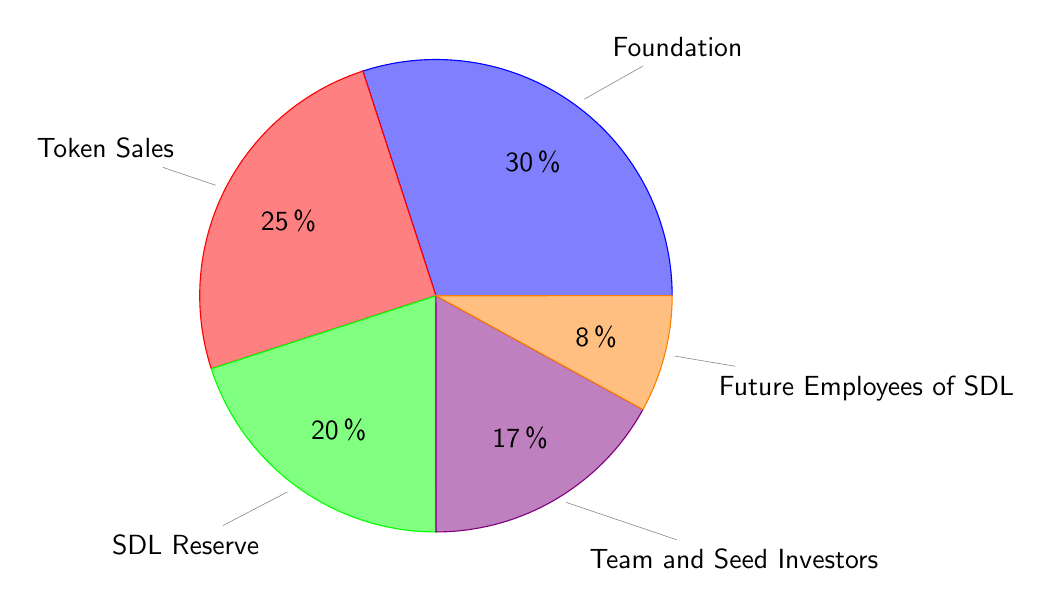
\begin{tikzpicture}[nodes = {font=\sffamily}]
    \foreach \percent/\name in {
          30/Foundation,
          25/Token Sales,
          20/SDL Reserve,
          17/Team and Seed Investors,
          8/Future Employees of SDL
        } {
          \ifx\percent\empty\else               % If \percent is empty, do nothing
            \global\advance\cyclecount by 1     % Advance cyclecount
            \global\advance\ind by 1            % Advance list index
            \ifnum4<\cyclecount                 % If cyclecount is larger than list
              \global\cyclecount=0              %   reset cyclecount and
              \global\ind=0                     %   reset list index
            \fi
            \pgfmathparse{\cyclelist[\the\ind]} % Get color from cycle list
            \edef\color{\pgfmathresult}         %   and store as \color
            % Draw angle and set labels
            \draw[fill={\color!50},draw={\color}] (0,0) -- (\angle:\radius)
              arc (\angle:\angle+\percent*3.6:\radius) -- cycle;
            \node at (\angle+0.5*\percent*3.6:0.7*\radius) {\percent\,\%};
            \node[pin=\angle+0.5*\percent*3.6:\name]
              at (\angle+0.5*\percent*3.6:\radius) {};
            \pgfmathparse{\angle+\percent*3.6}  % Advance angle
            \xdef\angle{\pgfmathresult}         %   and store in \angle
        \fi
        };
    \end{tikzpicture}
    \caption{Protocol token distribution breakdown. The total supply is capped at 13.5 billion.}
    \label{fig:TokenDistribution}
\end{figure}
The Protocol token (section \ref{section:Token} is capped to a total of 13.5 billion. The allocation of the token supply is given in figure \ref{fig:TokenDistribution}. The Protocol Foundation will be allocated the largest percentage of the supply at the time of token generation with Snickerdoodle Labs (SDL) receiving 20 percent of the supply.